\documentclass[
	letterpaper
	12pt
]{template}

\usepackage{apacite}
\usepackage{titling}
\usepackage{wrapfig}
\usepackage[font=footnotesize,labelfont=bf]{caption}

\setlength{\droptitle}{-10em}
\newcommand{\bref}[2]{\textbf{\hyperref[#1]{#2}}}

\begin{document}

\title{Motion in Fluids}

\author{Sebastien Psarianos, Yuchen Jiang}

\date{\today}
\maketitle
\section{Introduction}
This study explores the field of fluid dynamics by investigating how differing inertial and viscous force ratios, quantified in this experiment by Reynolds Number (\bref{eqn::reynolds}{Equation 1}), affect the drag force experienced by a falling object. Through terminal velocity analysis of spheres with differing sizes falling through both a high and low Reynolds number regime, we hope to provide a quantitative analysis of the accuracy of high and low Reynolds number approximations for drag force \bref{eqn::dragForce}{Equation 2}.

\subsection{Background}
Reynolds number (\bref{reynolds}{Equation 1}) is the measure used in this report to quantify whether a system's mechanics are dominated inertial or viscous forces. It is a dimensionless quantity that represents the ratio of inertial to viscous forces, defined as follows:
\begin{equation}\label{eqn::reynolds}
	R_e = \frac{\rho l v}{\eta}\ \ \text{\cite{batchelor_2002}}
\end{equation}
Where $\rho$ represents density $l$ is the objects size $v$ is its speed and $\eta$ is the fluid density. An object falling at terminal velocity can be modelled as the velocity where the drag force $F_d(v)$ and the gravitational force $mg$ are equal:
\[mg = F_d(v_{t})\]
Applying this terminal velocity condition to both an idealized high and low Reynolds number system, one can derive the following approximations for drag force in both regimes:
\begin{align}\label{eqn::dragForce}
	F_d(v) = 6\pi\eta r v \text{ (Low $R_e$)} && F_d(v) = {1\over 2}\rho C_dAv^2 \text{ (High $R_e$)} && \cite{labManual}
\end{align}
Where $C_d$ is an empirically measured drag coefficient, $\rho$ is fluid density, $A$ is cross-sectional area and $r$ is the object's radius. Rewriting the mass in terms of volume and density ($m =  {4\over 3}\rho_{\rm s}\pi r^3$), substituting $A=\pi r^2$ then solving for $v_{\rm term}$ gives the following predictions for terminal velocity:
\begin{align}\label{eqn::terminalVelocity}
	v_{\rm term}  = {2\rho_{\rm s} \over 9 \eta}\cdot r^2 \text{ (Low $R_e$)} && 	v_{term} =\sqrt{8\rho_{\rm s} g\over \rho C_d  3}\cdot \sqrt{r} \text{ (High $R_e$)}
	&& \cite{labManual}
\end{align}

\subsection{The experiment}
In this experiment we used glycerine to simulate our low Reynolds Number regime and water to simulate our high Reynolds Number regime. This choice was made due to water's low density $\eta_{w} \approx 1\times10^{-2}\unit{g\per {\cm\second}}$ in comparison to glycerine $\nu_g \approx 9.34\unit{g\per {\cm\second}}$ \cite{labManual}. Since \bref{eqn::reynolds}{Reynold's Number} is inversely related to fluid viscosity, water will have a comparatively larger Reynolds Number than  glycerine for a given velocity/size scale. By measuring terminal velocity of spheres of varying radii falling through both fluids, we aim to quantitatively examine the accuracy the terminal velocity predictions in \bref{eqn::terminalVelocity}{Equation 3}, derived from the drag force predictions in \bref{eqn::dragForce}{Equation 2}.


\section{Methodology}
\subsection{Apparatus}
\begin{wrapfigure}{r}{0.35\textwidth}\label{fig::apparatus}
	\centering
	\vspace{-10pt}
	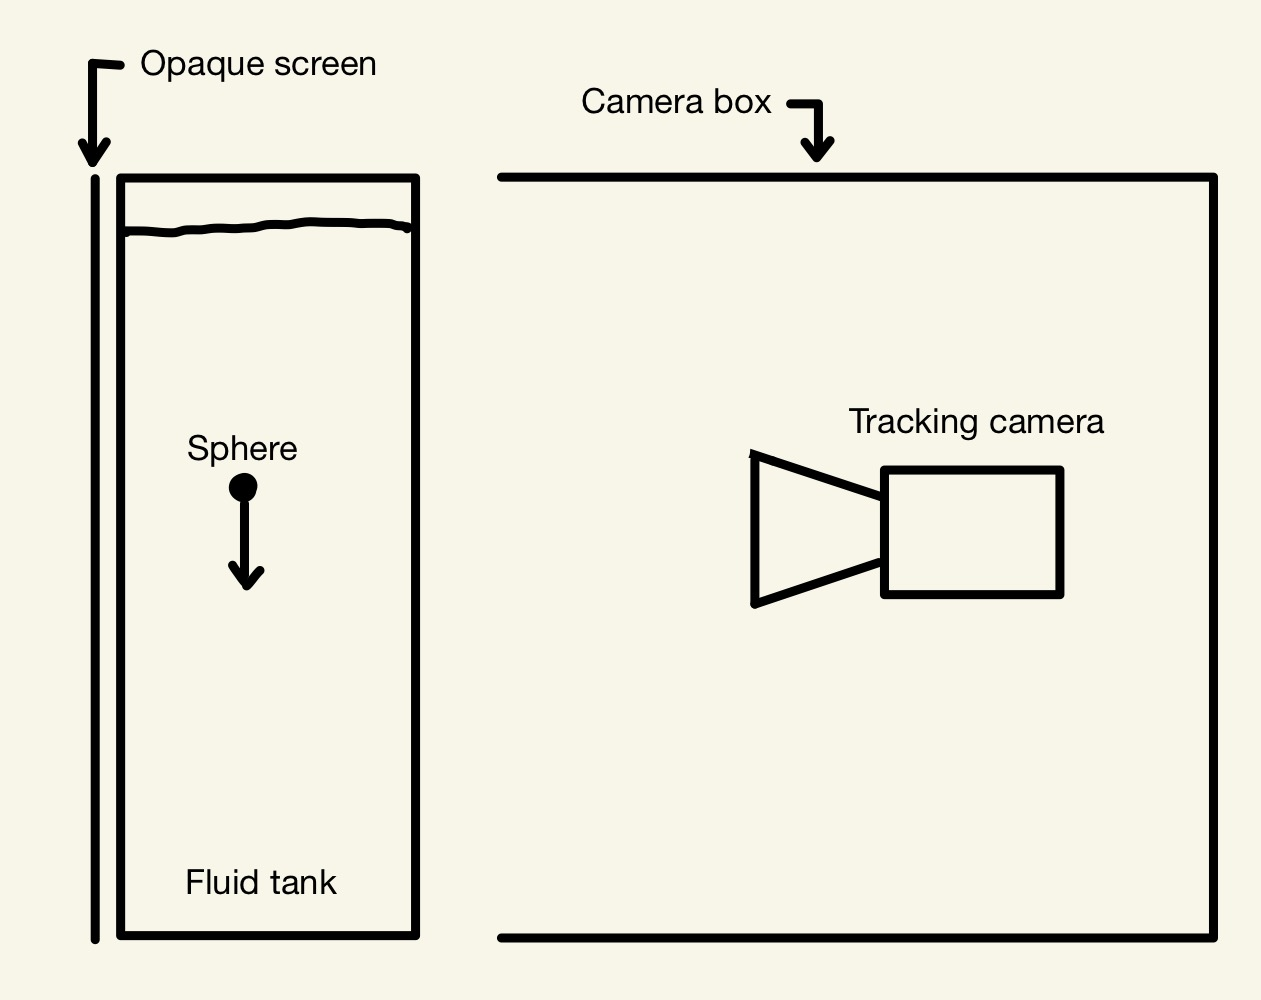
\includegraphics[width=.35\textwidth]{figures/apparatus.jpg}
	\caption{Diagram of apparatus}
	\vspace{-20pt}
\end{wrapfigure}
For each fluid, the terminal velocity of five differing size categories of beads were tested. Teflon beads were for the glycerine tank and Nylon beads were used for the water tank. These materials were chosen for their densities and minimal water absorption properties, allowing them to maintain consistent shape and weight during the experiment.\vspace{\baselineskip}

The vessel that was used to contain the fluid that was being tested was a transparent, rectangular tank. On one side of this container, an opaque screen was attached that completely covered that side of the container. The use of this screen in conjunction with the white color of the beads created a high contrast environment for optimal video tracking. \vspace{\baselineskip}

A camera was set up in an opaque box, opposing the opaque screen. There was an opening in the box that allowed the camera to view the interior of the tank. The camera's frame rate was changed in each trial to strike a balance between high time resolution and managing file sizes. A diagram of this apparatus is displayed in \bref{fig::apparatus}{Figure 1}. The video recording and tracking were performed using a purpose built LabView applet called "Motion through Fluids" provided with the apparatus.
\subsection{Procedure}
\subsubsection{Initial time estimates}\label{sec::timeEst}
Prior to starting the experiment, we dropped one bead from each of the five size categories into its corresponding fluid and timed how long it took to reach the bottom of the tank. This gave a rough estimate of how long each trial would take, informing the choice of video duration and frame rate for each sample.
\subsubsection{Trial Process}
For both fluids, we performed three trials for each of the 5 bead sizes, giving 15 total glycerine samples and 15 total water samples. The following procedure was followed for all of these trials: \vspace{\baselineskip}

First, the diameter of the bead was measured using a set of calipers. Since it was non-trivial to measure the widest part of the bead and determine the diameter, three measurements were taken for each bead and the largest value measured was the one that was used. Using the total decent time detailed in \bref{sec::timeEst}{2.2.1} determined for the specific bead-size/fluid combination, an appropriate frame count and frame-rate was chosen within the software. After the video tracking had been started in the software, the bead was carefully released in the center of the container using a set of tweezers. Once the video tracking process had ended, the LabView applet returned a text document containing the position vs time.
\vspace{\baselineskip}

Through the course pre-experimental trial runs, two adjustments were made to the process. Releasing the bead on top of the fluid gave a noticeable increase in test duration, likely due to surface tension. Therefore, care was taken to release the bead under the surface of the fluid to minimize these effects. Additionally, tracking tended to have issues tracking the bead right after it started. Therefore, the bead was released a short duration after the video had started, and this pre-drop data was removed after the fact.
\section{Results and Analysis}
\subsection{Calculating Terminal Velocity}
The data that was given by the LabView applet contained position values corresponding to specific timestamps. Therefore, to calculate the terminal velocity, some further processing was required. For every sample in both the glycerine and water trials, the following procedure was followed: First, the data was parsed from the output file of the Labview applet, giving a set of position time tuples. Then, for every set of two consecutive position time tuples, the average velocity between those two points was calculated using $v_{avg} = \Delta x/ \Delta t$. This gave $n-1$ velocity measurements (where $n$ is the number of position measurements directly from the software). From this set of velocity measurements, the largest value was chosen to be the terminal velocity and plotted using matplotlib. In addition to this, the function curve\_fit from the scipy.optimize module was used to perform a regression on both sets of terminal velocities. This was done using \bref{squaredFit}{Function 2} (the python implementation of  \bref{lowReynold}{Equation 3}) for the glycerine and \bref{sqrtFit}{Function 1}(the python implementation of  \bref{highReynold}{Equation 4}) for the water. The results of these plots are shown in \bref{terminalGlyc}{Figure 1} for the glycerine experiment and \bref{terminalWater}{Figure 3} for the water experiment.\\

In addition, for each sample, an overall average velocity was calculated for reference. This was done by taking the total displacement during the experiment and dividing it by the total time elapsed. This was also fit with the same model corresponding to the viscosity of the fluid. These plots are displayed in \bref{avgGlyc}{Figure 3} and \bref{averageWater}{Figure 4}.\\

In all the experiments, increased speed and / or smaller bead radius sometimes resulted in the tracking software losing the position of the particle. Due to this some filtering was done on the date to reduce this effect and provide a precise data set. This is discussed in more details in \bref{filtering}{Section 3.3}
\subsection {Resulting Graphs}
\begin{figure}[H]
	\begin{minipage}[t]{0.45\textwidth}\label{terminalGlyc}
		\centering
		\caption{Terminal velocity of a teflon bead falling through a glycerine tank (mm/s) vs bead radius (mm). Terminal velocity was measured by taking the average velocity over each time interval. These velocities were sorted, and the largest velocity was plotted for each sample. A fit is included of \bref{lowReynold}{Equation 3} (The low reynold number radius velocity relation approximation).}
		\includegraphics[width=0.9\textwidth]{../python/output/glycMaxFit.pdf}
	\end{minipage}
	\hfill
	\begin{minipage}[t]{0.45\textwidth}\label{avgGlyc}
		\centering
		\caption{Average velocity of a teflon bead falling through a glycerine tank (mm/s) vs bead radius (mm). Average velocity was calculated by taking the total distance traveled over the total time elapsed during the experiment. A fit is included of \bref{lowReynold}{Equation 3}. (The low reynold number radius velocity relation approximation)}
		\includegraphics[width=0.9\textwidth]{../python/output/glycSecFit.pdf}
	\end{minipage}
\end{figure}

\begin{figure}[H]
	\begin{minipage}[t]{0.45\textwidth}\label{terminalWater}
		\centering
		\caption{Terminal velocity of a nylon bead falling through a water tank (mm/s) vs bead radius (mm). Terminal velocity was measured by taking the average velocity over each time interval. These velocities were sorted, and the largest velocity was plotted for each sample. A fit is included of \bref{highReynold}{Equation 4} (The high reynold number radius velocity relation approximation).}
		\includegraphics[width=0.9\textwidth]{../python/output/waterMaxGraph.pdf}
	\end{minipage}
	\hfill
	\begin{minipage}[t]{0.45\textwidth}\label{averageWater}
		\centering
		\caption{Average velocity of a nylon bead falling through a water tank (mm/s) vs bead radius (mm). Average velocity was calculated by taking the total distance traveled over the total time elapsed during the experiment. A fit is included of \bref{highReynold}{Equation 4}. (The high reynold number radius velocity relation approximation)}
		\includegraphics[width=0.9\textwidth]{../python/output/waterSecGraph.pdf}
	\end{minipage}
\end{figure}
\subsection{Data Filtering}\label{filtering}
As discussed previously, the software would occasionally lose track the bead's position as the speed increased and the diameter decreased. This resulted in some data, especially in the water experiment having inaccurate position values. Due to this, the decision was made to make an effort to reduce the effect of these on the final data fits through filtering out these data points. This was done in two main ways.\\

The first thing we did was remove the position, time tuples with a position value of $0$. Considering that all data sets started with a position greater than $0$, this value was only recorded when the software lost track of the position. This was done prior to any velocity calculations described previously.\\

In addition, we plotted every calculated velocity for each sample to get a visualization of the terminal velocity We noticed that every sample had a clear trend to a terminal velocity. In addition, it could be seen that this terminal velocity was always less than 2.5 times the mean value. However, we also noticed that many plots had unrealistically large velocities that were frequently present. Therefore, we removed any velocity who's absolute value was greater than 2.5 times larger than the mean. After doing this, we reviewed the plots and noticed that for every sample, the terminal velocity trend was still completely present and none of these values were removed. Prior to this we were unsuccessful in performing a regression on the data set but after this, there were no more issues.
\subsection{Error Propagation}
All calculated terminal velocity values were calculated using the expression:
\[v_{avg} = {x_1-x_0\over t_1-t_0}\]
The time measurement was given an uncertainty of $\pm$ half of the frame interval, and the position measurement was given an uncertainty of half of the width of the particle. Therefore, the error propagation method that was used was to initially calculate the standard deviation of the "sums" $x_1-x_0$ and $t_1-t_0$ using \bref{addErr}{Equation 6}. Then these two uncertainties were propagated using the relative error propagation method for multiplication and division \bref{relErr}{Equation 5}.

\section{Conclusion}
This thorough investigation delves into the dynamics of fluids by examining the equilibrium, between viscous forces as measured through the Reynolds number. By conducting experiments that compare how quickly beads descend in Reynolds number settings (like glycerine) versus high Reynolds number settings (such as water) the study presents an analysis of how dominant forces influence fluid behavior. Using beads of sizes crafted from Teflon and Nylon researchers carefully monitor their descent through fluids with high speed video tracking enabling measurements of terminal velocities. The results confirm models for both high Reynolds numbers highlighting the significant impact of bead size and fluid viscosity on terminal velocities. This research not expands our comprehension of dynamics by offering empirical evidence to reinforce theoretical forecasts but also introduces a rigorous approach for filtering data and managing errors to ensure result accuracy. By determining Reynolds numbers under conditions this study provides valuable insights, into the core principles governing fluid movement thereby pushing forward the field of fluid mechanics and its practical implications.
\newpage
\appendix{}

\section{Summary of Equations}


\begin{minipage}[t]{0.45\textwidth}
	\begin{center}
		\begin{equation}
			\label{reynolds}
			Re = {\rho l v\over \eta}
		\end{equation}
		\textbf{Equation 1}: Definition of Reynolds Number
	\end{center}
\end{minipage}
\hfill1
\begin{minipage}[t]{0.45\textwidth}
	\begin{center}
		\begin{equation}
			\label{wallCorr}
			v_{corr } = v_m {1\over \left(1-2.104{d\over D} + 2.089\left({d\over D}\right)^3\right)}
		\end{equation}
		\textbf{Equation 2}: Correction factor used to account for wall effect \cite{labManual}
	\end{center}
\end{minipage}


\begin{minipage}[t]{0.45\textwidth}
	\begin{center}
		\begin{equation}
			\label{lowReynold}
			v_{\rm term}  = {2\rho_{\rm s} \over 9 \eta}\cdot r^2
		\end{equation}
		\textbf{Equation 3}: Low Reynold Approximation
	\end{center}
\end{minipage}
\begin{minipage}[t]{0.45\textwidth}
	\begin{center}
		\begin{equation}
			\label{highReynold}
			v_{term} =\sqrt{8\rho_{\rm s} g\over \rho C_d  3}\cdot \sqrt{r}
		\end{equation}
		\textbf{Equation 4}: High Reynold Approximation
	\end{center}
\end{minipage}


\begin{minipage}[t]{0.45\textwidth}
	\begin{center}
		\begin{equation}
			\label{relErr}
			{\Delta z\over z} = \sqrt{\left({\Delta x_i \over x_i}\right)^2 +...+ \left({\Delta x_i \over x_i}\right)^2}
		\end{equation}
		\textbf{Equation 5}: Relative Error approximation for multiplication and division
	\end{center}
\end{minipage}
\hfill
\begin{minipage}[t]{0.45\textwidth}
	\begin{center}
		\begin{equation}
			\label{addErr}
			\Delta z = \sqrt{\sum_{i=1}^n \Delta x_i^2}
		\end{equation}
		\textbf{Equation 6}: Variance formula for $z=\sum_{i=1}^n x_i$
	\end{center}
\end{minipage}

\section{Python Functions}

\begin{lstlisting}[caption={\label{sqrtFit}  Function used to fit the high reynolds number model \bref{highReynold}{Equation 4}},
captionpos=b,language=python]
def sqrtFit(x, A):
    return A * np.sqrt(np.abs(x))
\end{lstlisting}
\begin{lstlisting}[caption={\label{squaredFit}  Function used to fit the low reynolds number model \bref{lowReynold}{Equation 3}},
	captionpos=b,language=python]
def squaredFit(x, A):
	return A * x **2
\end{lstlisting}

\newpage
\bibliographystyle{apacite}
\bibliography{references.bib}
\end{document}
